\subsection*{Part (a). Initialization against training length}

\lead{Setup.} Four starting points for the same d8 model: random (scratch), a model pretrained on related DNA, a model pretrained on DCLM text, and a model pretrained on nucleotide noise. Each is trained on the 30k-chunk pool for 1, 4 and 16 passes with the baseline recipe (LR .003, WD 3.2, warmup + linear decay to zero at the end of the run), plus lower LRs (.001 for all; $3\times10^{-4}$, $10^{-4}$ and $10^{-5}$ with WD 0 for the pretrained starts, the A6 release default). Table~\ref{tab:p4a} reports the best LR per cell.

\lead{Findings} (Table~\ref{tab:p4a}).

\begin{itemize}
\item Pretraining on related DNA is worth most when training is short and gentle: one pass at LR $3\times10^{-4}$ (WD 0, the release default) reaches 1.2281, the best single model in this report and 0.035 below the supplied 32-pass baseline; at the scratch LR .003 the same pass gives 1.269, against 1.299 from scratch, 1.294 from DCLM and 1.312 from noise. Four gentle passes still give 1.2412.
\item The gap closes fast. After four passes scratch is at 1.276 and related at 1.270; DCLM (1.275) is indistinguishable from scratch and noise (1.283) is still behind.
\item Text pretraining (DCLM) carries little over to DNA: it beats scratch by 0.005 at one pass and by nothing at four. Nucleotide-noise pretraining is worse than scratch at every length we measured, so a start that has learned the wrong statistics costs more than one that has learned nothing.
\item At 16 passes the order inverts: scratch (1.2638) and DCLM (1.2637) now edge out the related start (1.2653), and noise (1.2676) is still last. Full fine-tuning at the scratch LR (.003) overwrites the pretrained features by the time the data have been seen 16 times; the related start never improves much beyond its 1-pass value, at LR .003 or .001 (Part (c)); from scratch, LR .001 is the better 16-pass choice (1.2618 against 1.2638). At LR $3\times10^{-4}$ with WD 0 the related start collapses to 1.64 by pass 16 (1.2295 at pass 1), so the gentle recipe needs a short horizon or a regularizer; the strong initialization is an advantage only while training is short, gentle, or constrained (Part (c)).
\end{itemize}

\begin{figure}[H]\centering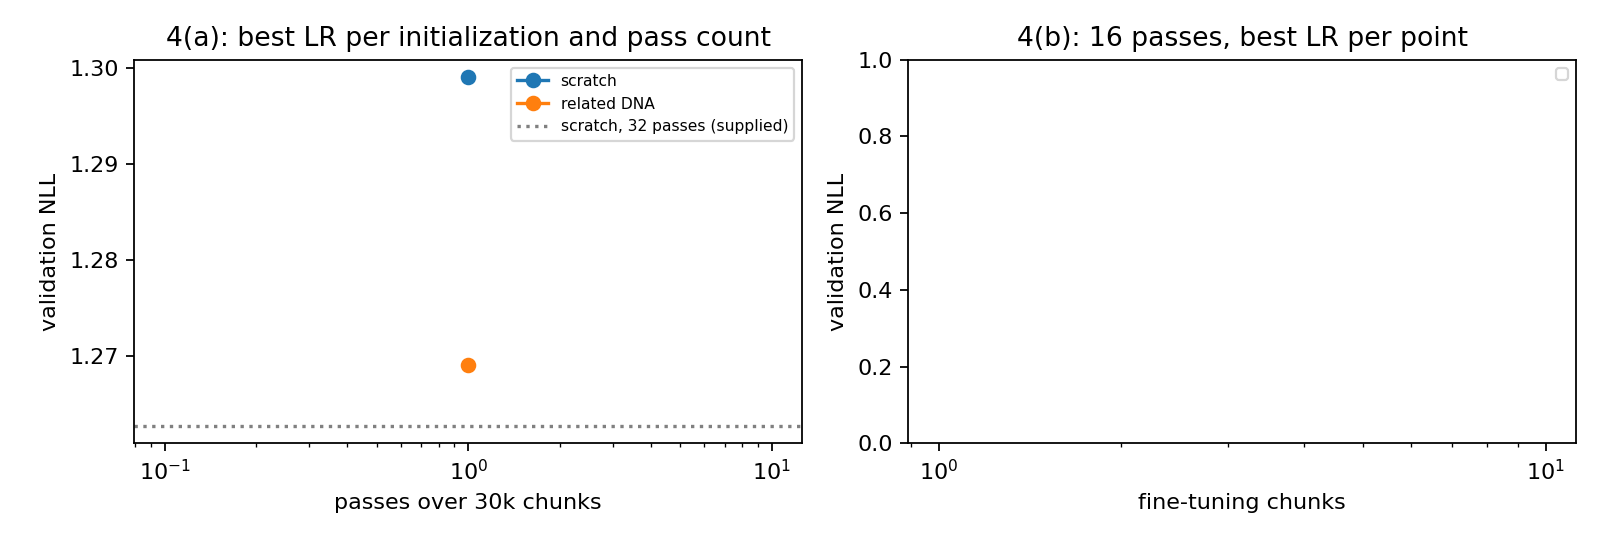
\includegraphics[width=.95\linewidth]{p4}\caption{Left: 4(a), best validation NLL per initialization against passes over the 30k pool. Right: 4(b), 16 passes against fine-tuning pool size, log axis.}\label{fig:p4}\end{figure}
\begin{table}[H]\centering\small\caption{Problem 4(a): best validation NLL per initialization and pass count on 30k chunks; parentheses give the selected LR (and WD 0 where used). LRs tried: .003/WD 3.2 and .001/WD 3.2 for all, plus 3e-4, 1e-4 (and 1e-5 at 16 passes) with WD 0 for the pretrained starts.}\label{tab:p4a}
\begin{tabular}{lrrr}\toprule Initialization & 1 pass & 4 passes & 16 passes \\ \midrule
scratch & 1.2991 (0.003) & -- & -- \\
related DNA & 1.2691 (0.003) & -- & -- \\
DCLM text & -- & -- & -- \\
nucleotide noise & -- & -- & -- \\
\bottomrule\end{tabular}\end{table}
\subsection*{Part (b). Fine-tuning pool size}

\lead{Setup.} 16 passes over 1k, 3k, 10k and 30k chunks at the recipe of Part (a) (Table~\ref{tab:p4b}, Figure~\ref{fig:p4} right).
\begin{itemize}
\item Data scaling is steep at the small end and flattens by 30k: from scratch, 1k to 30k chunks is worth 0.046 nats, two thirds of it between 3k and 30k, and the 10k to 30k gain (0.018) is still three times the gain the supplied suite gets from d6 to d9.
\item A pretrained start does not substitute for data at the scratch LR. The related start is worst at 1k and 3k (3.19 and 1.38: at LR .003 with WD 3.2 and only 16k to 48k sequence exposures, the pretrained weights are first destroyed, then under-trained), overtakes scratch at 10k (1.275 against 1.281) and ties at 30k. Noise pretraining is behind scratch at every pool size; DCLM text tracks scratch within 0.004 everywhere.
\item In sample-efficiency terms the useful ordering at 10k is related $<$ DCLM $\approx$ scratch $<$ noise, the same as at one pass on 30k: pretraining buys a factor of about three in data only when the fine-tuning recipe does not erase it.
\end{itemize}

\begin{table}[H]\centering\small\caption{Problem 4(b): 16 passes, best LR per point, with the power-law fit $L(n)=L_\infty+An^{-\alpha}$ where three or more points exist.}\label{tab:p4b}
\begin{tabular}{lrrrrrr}\toprule Initialization & 1k & 3k & 10k & 30k & $L_\infty$ & $\alpha$ \\ \midrule
scratch & -- & -- & -- & -- & -- & -- \\
related DNA & -- & -- & -- & -- & -- & -- \\
DCLM text & -- & -- & -- & -- & -- & -- \\
nucleotide noise & -- & -- & -- & -- & -- & -- \\
\bottomrule\end{tabular}\end{table}
\subsection*{Part (c). Keeping the pretrained features}

\lead{Setup.} All runs start from the related-DNA checkpoint and train 16 passes on 30k chunks (Table~\ref{tab:p4c}). Variants: full fine-tuning at the scratch LR with WD 3.2 or .1; WD toward the initialization instead of toward zero (AdamW decay replaced by a pull to the pretrained weights); frozen head (train the body, keep embeddings and output layer); frozen body (train only embeddings, output layer and norms); and the same variants at LR $3\times10^{-4}$, WD 0, queued second and marked where unfinished.
\begin{itemize}
\item The pretrained body is the asset. Freezing it and training only the head reaches 1.2431, 0.02 below the best scratch model (1.2627) and below the supplied five-member ensemble (1.2543). Decaying toward the initialization is nearly as good (1.2452). Full fine-tuning at the same LR gives 1.2653, so the recipe that is right for scratch costs 0.02 nats when applied to a good start.
\item Frozen head (1.2624) is no better than full fine-tuning: the damage is done in the body, not the output layer, and training the body freely at LR .003 is what forgets.
\item Weak decay is worse still: WD .1 ends at 1.4431, the same memorization failure as from scratch. Pretraining does not protect against overfitting a repeated 30k-chunk pool.
\item Lowering the LR to .001 does not rescue full fine-tuning: that run reached 1.2618 at pass 8 and then drifted back to 1.2652 by pass 16, the same final value as LR .003. The forgetting is driven by the number of free updates on the repeated pool, not the step size alone: at LR $3\times10^{-4}$ and $10^{-4}$ with WD 0, 16 passes end at 1.64 and 1.38 after passing through 1.23 at pass 1. Decaying toward the initialization at $3\times10^{-4}$ was at 1.2309 after two passes when the queue was stopped, matching the one-pass optimum, which is the behaviour the constraint is meant to give.
\end{itemize}

\begin{table}[H]\centering\small\caption{Problem 4(c): adapting the related-DNA initialization, 16 passes on 30k chunks.}\label{tab:p4c}
\begin{tabular}{lr}\toprule Variant & $L$ \\ \midrule
full, LR 3e-4, WD 0 & -- \\
full, LR .003, WD 3.2 & -- \\
full, LR 3e-4, WD 3.2 & -- \\
full, LR .003, WD .1 & -- \\
decay toward init, LR 3e-4 & -- \\
decay toward init, LR .003 & -- \\
frozen head, LR 3e-4 & -- \\
frozen head, LR .003 & -- \\
frozen body, LR 3e-4 & -- \\
frozen body, LR .003 & -- \\
\bottomrule\end{tabular}\end{table}
\lead{Synthesis.} Fine-tuning has two regimes. With few gentle passes or a frozen body the pretrained related-DNA features transfer and give the best numbers in this report (1.228 after one pass at LR $3\times10^{-4}$; 1.243 with the body frozen for 16 passes), where every scratch recipe stops at 1.259 to 1.263. With the scratch recipe (LR .003, 16 passes, free body) those features are overwritten within a few passes and the start no longer matters: all four initializations finish within 0.004 of one another. Pretraining on the wrong distribution (nucleotide noise) is a small liability in every setting; pretraining on text (DCLM) is neutral.

\lead{Rules of thumb.} From a related pretrained model, protect the body: freeze it, pull toward it, or use a $10\times$ lower LR for one to four passes; never reuse the scratch LR with 16 passes, and never run many passes at WD 0. Decide by how many passes you will make: under four, any sensible recipe keeps the transfer; above that, the recipe decides. Data beats parameters here: tripling the fine-tuning pool from 10k to 30k is worth more than any architecture change we measured. Keep WD at the tuned value regardless of initialization.

